\section{Warm Up: The Case of Two Tasks}\label{sec_defspike}


We would like to get insight on how covariate and model shifts affect the rate of transfer.
For the case of two tasks, we can get precise rates using random matrix theory.
For the sake of clarity, we call task 1 the source task and task 2 the target task,
i.e. $\beta_1 = \beta_s$ and $\beta_2 = \beta_t$.
%We denote task 1 as the source, i.e. $\beta_1 = \beta_s$.

\subsection{Covariate Shift}

As Proposition \ref{prop_monotone} shows, if $\beta_s$ and $\beta_t$ are equal, then adding the source task dataset always helps learn the target task.
The goal of this section is to understand how covariate shift affects the rate of transfer. \todo{add conceptual msg}

%The key quantity is to look at:
The estimator using the source and target together from minimizing \eqref{eq_mtl_basic} is
\[ \hat{\beta}_{s,t} = (X_1^{\top} X_1 + X_2^{\top} X_2)^{-1} (X_1^{\top}Y_1 + X_2^{\top}Y_2)\]
The estimation error of $\hat{\beta}_{s,t}$ is
\begin{align}\label{eq_two_task}
  \err(\hat{\beta}_{s,t}) = \sigma^2 \cdot \tr[(X_1^{\top}X_1 + X_2^{\top} X_2)^{-1}].
\end{align}
The estimation error using the target alone is
\begin{align}\label{eq_target_task}
	\err(\hat{\beta}_t) = \sigma^2 \cdot \tr[(X_2^{\top} X_2)^{-1}].
\end{align}
The improvement of estimation error from adding the source task is then given by
$\err(\hat{\beta}_t) - \err(\hat{\beta}_{s,t})$.
For the test error on the target task, the improvement from adding the source task is
\[ \te(\hat{\beta}_t) - \te(\hat{\beta}_{s,t}) = \sigma^2\cdot\bigtr{\bigbrace{(X_2^{\top}X_2)^{-1} - (X_1^{\top}X_1 + X_2^{\top}X_2)^{-1}}\cdot\Sigma_2}. \]

%We calculate the amount of improvement by comparing equation \eqref{eq_two_task} to equation \eqref{eq_target_task}.
We can get a precise result on the improvement of adding the source task data that only depends on the covariance matrices $\Sigma_1, \Sigma_2$ and the number of data points $n_1, n_2$.
We shall consider the high-dimensional setting such that
$$\gamma_n:= \frac{p} {n_1 + n_2} \to \gamma,\quad c_n:= \frac{n_1}{n_1 + n_2} \to c, \quad \text{as } \ n_1, n_2\to \infty, $$
for some constants $\gamma\in (0,\infty)$ and $c \in (0,1)$.

\begin{theorem}[Transfer rate under covariate shift]\label{thm_cov_shift}
	Let $\lambda_1, \lambda_2, \dots, \lambda_p$ denote the singular values of $\Sigma_1^{1/2}\Sigma_2^{-1/2}$.
	When there is no model shift, we have that
	\begin{align*}
		\err(\hat{\beta}_{s,t}) &= \sigma^2 p \cdot \bigtr{\frac 1 {(n_1 + n_2)a_1\Sigma_1 + (n_1 + n_2)a_2\Sigma_2}} \\
		\te(\hat{\beta}_{s,t}) &= \sigma^2 p \cdot \bigtr{\frac 1 {(n_1 + n_2)a_1\Sigma_2^{-1/2}\Sigma_1\Sigma_2^{-1/2} + (n_1 + n_2)a_2\id}}
	\end{align*}
	where $a_1, a_2$ are the solutions of the following equations
	\begin{gather}
		 a_1 + a_2 = 1- \frac{p}{n_1 + n_2} \label{eq_a1}\\
		 a_1 + \sum_{i=1}^p \frac{a_1}{(n_1 + n_2)a_1 + (n_1 + n_2)\lambda_i^2 a_2} = \frac{n_2}{n_1 + n_2}. \label{eq_a2}
	\end{gather}
\end{theorem}

\todo{redo the following}
As a remark, we see that Proposition \ref{prop_monotone} follows from Theorem \ref{thm_cov_shift}.
The amount of reduction on estimation error and test error for the target task is given as
	\begin{align*}
		\err(\hat{\beta}_t) - \err(\hat{\beta}_{s,t})
		&= \sigma^2 p \cdot \bigtr{\frac 1 {(n_2 - p) \Sigma_2} - \frac 1 {(n_1 + n_2)a_1 \Sigma_1 + (n_1 + n_2)a_2 \Sigma_2}}, \\
		\te(\hat{\beta}_t) - \te(\hat{\beta}_{s,t})
		&= \sigma^2 p \cdot \bigtr{\frac 1 {n_2 - p} - \frac 1 {(n_1 + n_2)a_1\Sigma_2^{-1/2}\Sigma_1\Sigma_2^{-1/2} + (n_1 + n_2)a_2\id}}.
	\end{align*}
Because
\begin{align*}
	\err(\hat{\beta}_{s,t}) \le \err(\hat{\beta}_t)
	\Leftarrow~ & (n_2 - p)\Sigma_2 \preceq (n_1 + n_2) a_1 \Sigma_1 + (n_1 + n_2)a_2 \Sigma_2 \\
	\Leftrightarrow~ & \zeroMatrix \preceq (n_1 + n_2) a_1 \Sigma_1 + (n_1 - (n_1 + n_2)\cdot a_1) \Sigma_2,
\end{align*}
which is true since $a_1 \le n_1 / (n_1 + n_2)$ by equation \eqref{eq_a2}.
The proof for $\te(\hat{\beta}_{s,t}) \le \te(\hat{\beta}_t)$ follows by multiplying $\Sigma_2^{-1/2}$ on both sides of the inequalities above.

Now we apply Theorem \ref{thm_cov_shift} to show how covariate shift affects the rate of transfer.

\paragraph{Example 1: when $\Sigma_1 = \Sigma_2$.}
In this case, we have $\lambda_i = 1$ for all $1\le i\le p$.
And $a_1 + a_2 = 1 - p / (n_1 + n_2)$.
Hence
\[ \te(\hat{\beta}_{s,t}) = \frac{\sigma^2 p^2}{n_1 + n_2 - p} \text{ and } \err(\hat{\beta}_{s,t}) = \frac {\sigma^2 p} {n_1 + n_2 - p} \bigtr{\Sigma_2^{-1}}. \]

\paragraph{Example 2: when $\Sigma_1 = \Sigma_2 / \lambda$.}
In this case, equations \eqref{eq_a1} and \eqref{eq_a2} become
\[ a_1 + a_2 = 1 - p/(n_1 + n_2), a_1 + \frac{p}{n_1 + n_2} \cdot \frac {a_1} {a_1 + \lambda^2 a_2} = \frac{n_1} {n_1 + n_2}. \]
By solving these, we can get the test errors (the estimation error behaves similarly).
Figure \ref{fig_te_scaling} shows how they grow as we increase the number of source task data points.
Here $n_2 = 4p$ and $n_1$ ranges from $p$ to $20p$.
We can see that the smaller $\lambda$ is, the lower the test errors will be.

\paragraph{Example 3: when $\Sigma_1$ and $\Sigma_2$ are complementary.}
Here we have that for $\Sigma_1^{-1/2}\Sigma_2^{1/2}$, the first $p/2$ singular values of $\Sigma_1$ is $\lambda$ and the rest is $1/\lambda$.
For this case, equations \eqref{eq_a1} and \eqref{eq_a2} become
\[ a_1 + a_2 = 1 - \frac{p}{n_1 + n_2}, a_1 + \frac{p}{2(n_1 + n_2)}\cdot \bigbrace{\frac{a_1}{a_1 + \lambda^2 a_2} + \frac{a_1}{a_1 + \frac{a_2}{\lambda^2}}} = \frac{n_1}{n_1 + n_2}. \]
It's not hard to verify that there is only one valid solution from the above.
After solving these, we get the test error for the target task as follows.
\[ \frac{p}{2(n_1 + n_2)} \cdot \bigbrace{\frac{1}{\frac{a_1}{\lambda^2} + a_2} + \frac{1}{a_1\lambda^2 + a_2}}.\]

In Figure \ref{fig_te_complement}, we plot the test error of the target task for $n_2 = 4p$ and $n_1$ ranging from $p$ to $20p$.
We observe the following two phases as we increase $n_1 / p$.
\begin{itemize}
	\item When $n_1 \le n_2$, having complementary covariance matrices leads to lower test error compared to the case when $\Sigma_1 = \Sigma_2$.
	\item When $n_1 > n_2$, having complementary covariance matrices leads to higher test error compared to the case when $\Sigma_1 = \Sigma_2$.
\end{itemize}

\begin{figure}
	\centering
	\begin{minipage}{0.48\textwidth}
		\centering
		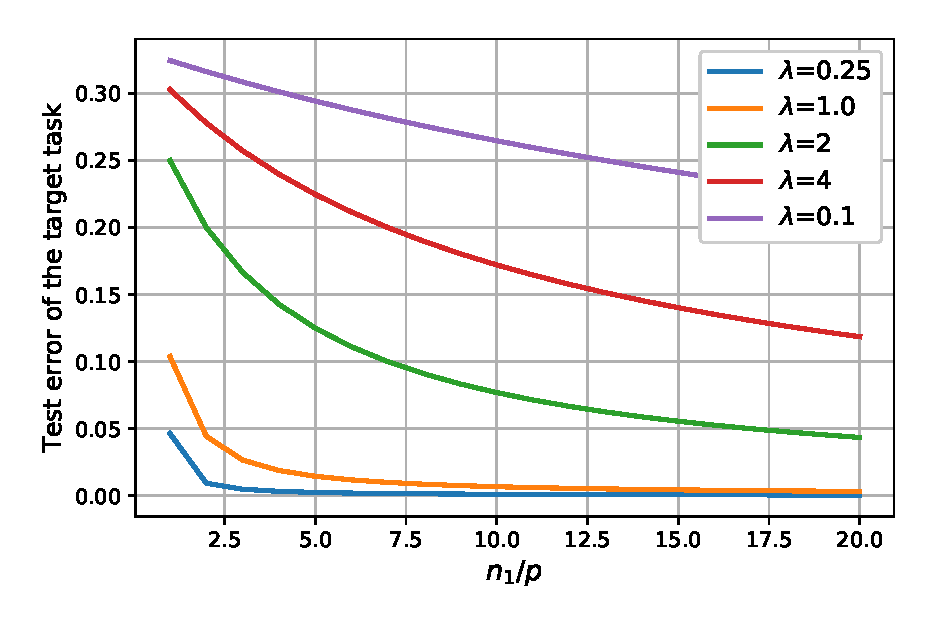
\includegraphics[width=0.9\textwidth]{figures/scaling.eps}
		\caption{When $\Sigma_1 = \Sigma_2 / \lambda$.}
		\label{fig_te_scaling}
	\end{minipage}\hfill
	\begin{minipage}{0.48\textwidth}
		\centering
		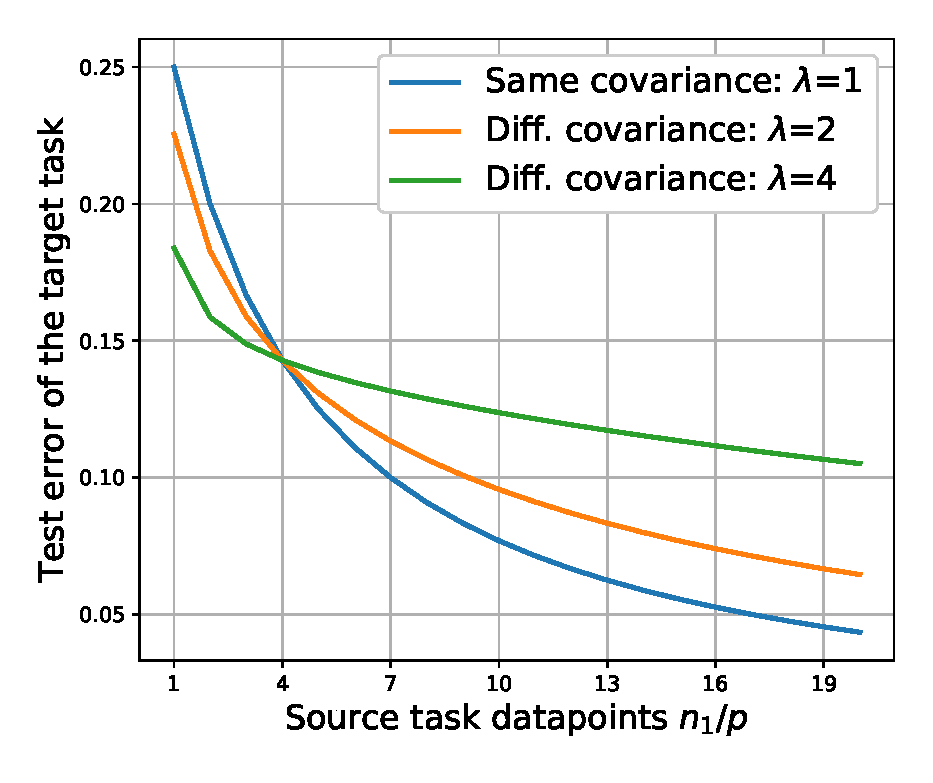
\includegraphics[width=0.9\textwidth]{figures/complementary.eps}
		\caption{When $\Sigma_1$ and $\Sigma_2$ are complementary.}
		\label{fig_te_complement}
	\end{minipage}
\end{figure}

\bigskip
To prove Theorem \ref{thm_cov_shift}, we study the spectrum of the random matrix model:
$$Q= \Sigma_1^{1/2}  Z_1^T Z_1 \Sigma_1^{1/2}  + \Sigma_2^{1/2}  Z_2^T Z_2 \Sigma_2^{1/2} ,$$
where $\Sigma_{1,2}$ are $p\times p$ deterministic covariance matrices, and $X_1=(x_{ij})_{1\le i \le n_1, 1\le j \le p}$ and $X_2=(x_{ij})_{n_1+1\le i \le n_1+n_2, 1\le j \le p}$ are $n_1\times p$ and $n_2 \times p$ random matrices, respectively, where the entries $x_{ij}$, $1 \leq i \leq n_1+n_2\equiv n$, $1 \leq j \leq p$, are real independent random variables satisfying
\begin{equation}\label{eq_12moment} %\label{assm1}
\mathbb{E} z_{ij} =0, \ \quad \ \mathbb{E} \vert z_{ij} \vert^2  = n^{-1}.
\end{equation} 
For now, we assume that the random variables $x_{ij}$ are i.i.d. Gaussian, but we know that universality holds for generally distributed entries. %have arbitrarily high moments, 
%in the sense that for any fixed $k\in \mathbb N$, there is a constant $\mu_k>0$ such that
%\begin{equation}\label{eq_highmoment} %\label{eqn:subgaus}
%\max_{i,j}\left(\mathbb E|x_{ij}|^k\right)^{1/k} \le \mu_k n^{-1/2},  %\var \left(h_{xy}\right)^{1/2}
%\end{equation}
%for all $n$. %For simplicity, we assume that $k$ is a finite fixed integer, the strengths $d_1 > d_2 > \cdots > d_k >0$ are fixed constants, and $ \bu_i$,  $\bv_i$ are deterministic unit vectors. 


\begin{lemma}\label{lem_cov_shift}
	In the setting of Theorem \ref{thm_cov_shift}, we have with high probability $1-{\rm o}(1)$,
\begin{align*}
\tr ((X_1^{\top}X_1 + X_2^{\top}X_2)^{-1}) = \frac{p}{n_1+n_2}\cdot \tr \left[ \frac{1}{a_1\Sigma_1 + a_2\Sigma_2} \right] +\bigo{\frac{p}{n^{1-\epsilon}}}.
\end{align*}
	for any constant $\epsilon>0$. %, where $a_{3,4}$ are found using equations in  \eqref{m35reduced}.
	In particular, when $n_1 = 0$, we have that $a_1 = 0$ and $a_2 = (n_2-p) / n_2$, hence
	\[ \bigtr{(X_2^{\top}X_2)^{-1}} = \frac{p}{n_2-p}\bigtr{\frac 1 {\Sigma_2}} + \bigo{\frac{p}{n_2^{1-\varepsilon}}}. \]
\end{lemma}

\todo{shift $\lambda$} We assume that $ \Sigma_1^{-1/2}\Sigma_2$ has eigendecomposition
\be  \label{eigen}
\Sigma_1^{-1/2}\Sigma_2^{1/2} = ODO^T ,\quad D=\text{diag}(d_1, \cdots, d_p).
\ee
Then by the rotational invariance of Gaussian matrices, we have
$$\wt Q \overset{d}{=}\Sigma_1^{1/2} O \wt Q O^T \Sigma_1^{1/2},\quad \wt Q:=   X_1^T X_1  + D X_2^T X_2 D .$$
Thus we study the spectrum of $\wt Q$ instead. We define $\cal G(z):= (\wt Q-z)^{-1}$ for $z\in \C_+$. With some random matrix tools, we have that 
$$\cal G(z) \approx \diag\left( \frac{1}{-z\left( 1+ m_3(z) + d_i^2 m_4(z)\right)}\right)_{1\le i \le p}= \frac{1}{-z\left( 1+ m_3(z) + D^2 m_4(z)\right)} $$
{\cob in certain sense}. Here $m_{3,4}(z)$ satisfy the following self-consistent equations
%$$\frac{1}{G_{ii}} \approx -z \left( 1+m_3 + d_i^2m_4 \right), \quad \frac{1}{G_{\mu\mu}} = -z(1+m_1), \ \ \mu\in \cal I_1,\quad \frac{1}{G_{\nu\nu}} = -z(1+m_2), \ \ \nu\in \cal I_2,$$
%$$m_1= \frac1n\sum_{i}G_{ii}, \quad m_2= \frac1n\sum_{i}d_i^2 G_{ii}, \quad m_3 = \frac1n\sum_{\mu\in \cal I_1} G_{\mu\mu},\quad m_4 = \frac1n\sum_{\mu\in \cal I_2} G_{\mu\mu}.$$
\begin{align}\label{m34}
\frac{n_1}{n}\frac1{m_3} = - z +\frac1n\sum_{i=1}^p \frac1{  1+m_3 + d_i^2m_4  } ,\quad \frac{n_2}{n}\frac1{m_4} = - z +\frac1n\sum_{i=1}^p \frac{d_i^2 }{  1+m_3 + d_i^2m_4  } 
\end{align}
When $z\to 0$, we shall have
$$m_3(z)= - \frac{a_3}{z} + \OO(1), \quad m_4(z)= - \frac{a_4}{z} + \OO(1),\quad a_3,a_4>0.$$
Then for $z\to0$, the equations in \eqref{m34} are reduced to
\begin{align}\label{m35}
\frac{n_1}{n}\frac{1}{a_3} = 1 +\frac1n\sum_{i=1}^p \frac{1}{a_3 + d_i^2a_4  } ,\quad \frac{n_2}{n}\frac1{a_4} = 1 +\frac1n\sum_{i=1}^p \frac{d_i^2 }{  a_3 + d_i^2 a_4 }. 
\end{align}
First, it is easy to see that these equations are equivalent to
\begin{align} a_3 + a_4 = 1- \gamma_n, \quad a_3 +\frac1n\sum_{i=1}^p \frac{a_3}{a_3 + d_i^2[(1-\gamma_n)-a_3]  }=c_n  .\end{align}
Furthermore, we have
\begin{align*}
\tr (Q^{-1}) &= \lim_{z\to 0}\tr \left[\Sigma_1^{-1/2} O \cal G(z)O^T \Sigma_1^{-1/2}\right]
=\tr \left[\Sigma_1^{-1/2} O  \left( \frac{1}{a_3 + D^2 a_4 }\right) O^T \Sigma_1^{-1/2}\right] \\
&=\tr \left[\Sigma_1^{-1/2}  \frac{1}{a_3+ \Sigma_1^{-1}\Sigma_2 a_4} \Sigma_1^{-1/2}\right]=\tr \left[ \frac{1}{a_3\Sigma_1 + a_4\Sigma_2 } \right].
\end{align*}

\subsection{Model Shift}

In this case, $\beta_s$ and $\beta_t$ are different.
From \cite{WZR20}, we know that either we need to explicitly restrict the capacity $r$ of $B$, or implicitly add a regularization on $B$.
\todo{We focus on the former case in this section.}
Following \cite{WZR20}, we consider the case when $r=1$ since there are only two tasks.

\subsubsection{The Objective with Shared Weights}

We begin by considering the simplified equation \eqref{eq_mtl_basic} to solve for the target task.
By putting the two tasks together, we get
\begin{align*}
	\hat{\beta}_{s,t} &= (X_1^{\top}X_1 + X_2^{\top}X_2)^{-1} (X_1^{\top}Y_1 + X_2^{\top}Y_2) \\
	&= (X_1^{\top}X_1 + X_2^{\top}X_2)^{-1} \bigbrace{(X_1^{\top}X_1\beta_s + X_2^{\top}X_2\beta_t) + (X_1^{\top}\varepsilon_1 + X_2^{\top}\varepsilon_2)} \\
	&= \beta_t + (X_1^{\top}X_1 + X_2^{\top}X_2)^{-1}\bigbrace{X_1^{\top}X_1(\beta_s - \beta_t) + (X_1^{\top}\varepsilon_1 + X_2^{\top}\varepsilon_2)}
\end{align*}
Hence
\begin{align}
	\err(\hat{\beta}_{s,t})
	&= \bignorm{(X_1^{\top}X_1 + X_2^{\top}X_2)^{-1} X_1^{\top}X_1 (\beta_s - \beta_t)}^2
	+ \sigma^2 \bigtr{(X_1^{\top}X_1 + X_2^{\top}X_2)^{-1}}, \text{ and} \\
	\te(\hat{\beta}_{s,t})
	&= \bignorm{\Sigma_2^{1/2} (X_1^{\top}X_1 + X_2^{\top}X_2)^{-1} X_1^{\top}X_1 (\beta_s - \beta_t)}^2 + \sigma^2\cdot \bigtr{(X_1^{\top}X_1 + X_2^{\top}X_2)^{-1}\Sigma_2}
\end{align}

We can see that because of model shift, i.e. $\beta_s \neq \beta_t$.
We can no longer guarantee that $\te(\hat{\beta}_{s,t}) \le \te(\hat{\beta}_t)$.
The goal of this part is to show conditions under which we get positive vs. negative transfer.

\todo{For technical reasons, we will consider the test error.} From Lemma \ref{lem_cov_shift}, we know that
\[ \bigtr{(X_1^{\top}X_1 + X_2^{\top}X_2)^{-1} \Sigma_2} = \frac{p}{n_1 + n_2}\cdot \bigtr{ \bigbrace{a_1\Sigma_2^{-1/2}\Sigma_1\Sigma_2^{-1/2} + a_2\id}^{-1}}, \]
where $a_1, a_2$ are specified in Theorem \ref{thm_cov_shift}.
It remains to consider the first term in $\te(\hat{\beta}_{s,t})$, which is bounded using the following lemma.
%We are now interested in the following quantity

\begin{theorem}[Positive transfer under model shift]
	a
\end{theorem}

\begin{theorem}[Negative transfer under model shift]
\end{theorem}

\begin{lemma}
	\todo{check}
	Let $a_1, a_2$ be the solutions from equations \eqref{eq_a1} and \eqref{eq_a2}.
	Denote by $M \define \Sigma_1^{1/2}\Sigma_2^{-1/2}$.
	\todo{The following?}
	\begin{align*}
		&~ \bignorm{\Sigma_2^{1/2} (X_1^{\top}X_1 + X_2^{\top}X_2)^{-1}X_1^{\top}X_1(\beta_s - \beta_t)}^2 \\
		\le &~ (\beta_s - \beta_t)^{\top} \Sigma_1^{1/2} M \frac{(1 + a_3)\id + a_4 M^{\top}M}{(a_1 + a_2 M^{\top}M)^2} M^{\top} \Sigma_1^{1/2} (\beta_s - \beta_t)
	\end{align*}


	We have that
	\begin{align*}
		&~ {\bignorm{\Sigma_2^{1/2} (X_1^{\top}X_1 + X_2^{\top}X_2)^{-1} X_1^{\top}X_1 (\beta_s - \beta_t)}} \\
		&\le ~ \left[(\beta_s - \beta_t)^{\top}\Sigma_1^{1/2}M\frac{(1 + a_3)\id + a_4 M^{\top}M}{(a_1 + a_2 M^{\top}M)} M^{\top}\Sigma_1^{1/2} (\beta_s - \beta_t)\right]^{1/2} \\
		&+ \left\|M\frac{(1 + a_3)\id + a_4 M^{\top}M}{(a_1 + a_2 M^{\top}M)} M^{\top}\right\|_{op}^{1/2} \|\Sigma_1^{1/2} (\beta_s - \beta_t)\|_2 \left( 2\sqrt{\frac{p} {n_1}} + \frac{p}{n_1}\right),
	\end{align*}
	and
	\begin{align*}
		&~ {\bignorm{\Sigma_2^{1/2} (X_1^{\top}X_1 + X_2^{\top}X_2)^{-1} X_1^{\top}X_1 (\beta_s - \beta_t)}} \\
		&\ge ~ \left[(\beta_s - \beta_t)^{\top}\Sigma_1^{1/2}M\frac{(1 + a_3)\id + a_4 M^{\top}M}{(a_1 + a_2 M^{\top}M)} M^{\top}\Sigma_1^{1/2} (\beta_s - \beta_t)\right]^{1/2} \\
		&- \left\|M\frac{(1 + a_3)\id + a_4 M^{\top}M}{(a_1 + a_2 M^{\top}M)} M^{\top}\right\|_{op}^{1/2} \|\Sigma_1^{1/2} (\beta_s - \beta_t)\|_2 \left( 2\sqrt{\frac{p} {n_1}} + \frac{p}{n_1}\right).
	\end{align*}
	Here in the error term $p$ can be replaced with the rank of $\Sigma_1$. Without any extra information, we can only use the fact the rank of $\Sigma_1$ is at most $p$.
	
	Here $a_3, a_4$ are the solutions of the following linear equations
%	\begin{align}
%		\left(\frac{n_2}{n_1+n_2}\frac1{a_1^2}- \frac1{n_1+n_2}\sum_{i=1}^p \frac{1}{ (a_1 + \lambda_i^2a_2)^2  }\right) a_3 -  \left(\frac1{n_1+n_2}\sum_{i=1}^p \frac{  \lambda_i^2 }{ (  a_1 + \lambda_i^2a_2)^2  }\right)a_4 &=  \frac1{n_1+n_2}\sum_{i=1}^p \frac{1 }{ (  a_1 + \lambda_i^2a_2)^2  } , \label{eq_a3} \\
%		\left( \frac{n_1}{n_1+n_2}\frac1{a_2^2} -  \frac1n\sum_{i=1}^p \frac{\lambda_i^4   }{  (a_1 + \lambda_i^2a_2)^2  }\right)a_4 -\left( \frac1 {n_1+n_2}\sum_{i=1}^p \frac{\lambda_i^2  }{  (a_1 + \lambda_i^2a_2)^2  }\right)a_3 &=   \frac1 {n_1+n_2}\sum_{i=1}^p \frac{\lambda_i^2 }{  (a_1 + \lambda_i^2a_2)^2  }. \label{eq_a4}
%	\end{align}	
	\begin{align}
		\left( \frac1{a_1^2}- \frac1{n_2}\sum_{i=1}^p \frac{1}{ (a_1 + \lambda_i^2a_2)^2  }\right) a_3 -  \left(\frac1{n_2}\sum_{i=1}^p \frac{  \lambda_i^2 }{ (  a_1 + \lambda_i^2a_2)^2  }\right)a_4 &=  \frac1{n_2}\sum_{i=1}^p \frac{1 }{ (  a_1 + \lambda_i^2a_2)^2  } , \label{eq_a3} \\
		\left( \frac1{a_2^2} -  \frac1{n_1}\sum_{i=1}^p \frac{\lambda_i^4   }{  (a_1 + \lambda_i^2a_2)^2  }\right)a_4 -\left( \frac1 {n_1}\sum_{i=1}^p \frac{\lambda_i^2  }{  (a_1 + \lambda_i^2a_2)^2  }\right)a_3 &=   \frac1 {n_1}\sum_{i=1}^p \frac{\lambda_i^2 }{  (a_1 + \lambda_i^2a_2)^2  }. \label{eq_a4}
	\end{align}
\end{lemma}

We consider the same setting as in previous subsection: 
$$ X_1^{\top}X_1:=\Sigma_1^{1/2}  Z_1^T Z_1 \Sigma_1^{1/2} ,\quad X_2^{\top}X_2= \Sigma_2^{1/2}  Z_2^T Z_2 \Sigma_2^{1/2},$$
where $z_{ij}$, $1 \leq i \leq n_1+n_2\equiv n$, $1 \leq j \leq p$, are real independent random variables satisfying \eqref{eq_12moment}. For now, we assume that the random variables $z_{ij}$ are i.i.d. Gaussian, but we know that universality holds for generally distributed entries. Assume that $p/n_1$ is a small number such that $Z_1^TZ_1$ is roughly an isometry, that is, under \eqref{eq_12moment}, 
\todo{
\begin{align}\left\| Z_1^T Z_1 -  \frac{n_1}{n} I \right\| \le 2\sqrt{\frac{p}{n}} + {\frac{p}{n}} .
\end{align}}
{\color{blue}
If we assume the variances of the entries of $Z_1$ are $p^{-1}$, then we have
\begin{align}
-\frac{n_1}{p}\left(2\sqrt{\frac{p}{n_1}} - {\frac{p}{n_1}}\right)  \le Z_1^T Z_1 -  \frac{n_1}{p} I  \le \frac{n_1}{p}\left(2\sqrt{\frac{p}{n_1}} + {\frac{p}{n_1}}\right) .
\end{align}
}

Then we have
$$  \left\|X_1^{\top}X_1 (\beta_s - \beta_t)  - \frac{n_1}{n}(\beta_s - \beta_t)\right\|_2 \le C \sqrt{\frac{p}{n}} \left\| (\beta_s - \beta_t)\right\|_2. $$
It remain to study the following expression 
\begin{align*}
\frac{1}{X_1^{\top}X_1 + X_2^{\top}X_2}  \Sigma_2 \frac{1}{X_1^{\top}X_1 + X_2^{\top}X_2}  = \Sigma_2^{-1/2}\left(\frac{1}{A^T Z_1^{\top}Z_1 A + Z_2^{\top}Z_2} \right)^2 \Sigma_2^{-1/2} \\
\stackrel{d}{=} \Sigma_2^{-1/2}V \left(\frac{1}{\Lambda Z_1^{\top}Z_1 \Lambda + Z_2^{\top}Z_2} \right)^2 V^T \Sigma_2^{-1/2},
\end{align*}
where 
\be  \label{eigen2}
A:=\Sigma_1^{1/2}\Sigma_2^{-1/2} = U\Lambda V^T ,\quad \Lambda=\text{diag}(\lambda_1, \cdots, \lambda_p).
\ee
Using 
$$\left(\frac{1}{\Lambda Z_1^{\top}Z_1 \Lambda + Z_2^{\top}Z_2} \right)^2 =\left. \frac{\dd }{\dd z}\right|_{z=0}\frac{1}{\Lambda Z_1^{\top}Z_1 \Lambda + Z_2^{\top}Z_2 - z} ,$$
we  need to study the resolvent of 
$$G(z) = \left( \Lambda Z_1^{\top}Z_1 \Lambda + Z_2^{\top}Z_2 - z \right)^{-1}.$$
Its local law can be studied as in previous subsection (be careful we need to switch the roles of $Z_1$ and $Z_2$). More precisely,  we have that 
$$ G(z) \approx \diag\left( \frac{1}{-z\left( 1+ m_3(z) + \lambda_i^2 m_4(z)\right)}\right)_{1\le i \le p}= \frac{1}{-z\left( 1+ m_3(z) + \Lambda^2 m_4(z)\right)} .$$
Here $m_{3,4}(z)$ satisfy the following self-consistent equations
%$$\frac{1}{G_{ii}} \approx -z \left( 1+m_3 + d_i^2m_4 \right), \quad \frac{1}{G_{\mu\mu}} = -z(1+m_1), \ \ \mu\in \cal I_1,\quad \frac{1}{G_{\nu\nu}} = -z(1+m_2), \ \ \nu\in \cal I_2,$$
%$$m_1= \frac1n\sum_{i}G_{ii}, \quad m_2= \frac1n\sum_{i}d_i^2 G_{ii}, \quad m_3 = \frac1n\sum_{\mu\in \cal I_1} G_{\mu\mu},\quad m_4 = \frac1n\sum_{\mu\in \cal I_2} G_{\mu\mu}.$$
\begin{align}\label{m34shift}
\frac{n_2}{n}\frac1{m_3} = - z +\frac1n\sum_{i=1}^p \frac1{  1+m_3 + \lambda_i^2m_4  } ,\quad \frac{n_1}{n}\frac1{m_4} = - z +\frac1n\sum_{i=1}^p \frac{\lambda_i^2 }{  1+m_3 + \lambda_i^2m_4  } .
\end{align}
Then we calculate the derivatives of $u_3:=zm_3$ and $u_4:=zm_4$ with respect to $z$:
\begin{align}\label{dotm34}
\frac{n_2}{n}\frac1{u_3^2}u'_3 =  \frac1n\sum_{i=1}^p \frac{1+u'_3 + \lambda_i^2 u'_4}{ ( z+u_3 + \lambda_i^2u_4)^2  } ,\quad \frac{n_1}{n}\frac1{u_4^2}u'_4 =   \frac1n\sum_{i=1}^p \frac{\lambda_i^2\left(1+u'_3 + \lambda_i^2 u'_4\right) }{  (z+u_3 + \lambda_i^2u_4)^2  } .
\end{align}
We can solve the above equations to get $u'_3$ and $u'_4$. Then we have 
$$ G^2(z) \approx   \frac{1 +  u_3'(z) +\Lambda^2 u'_4(z)}{ \left( z+ u_3(z) + \Lambda^2  u_4(z)\right)^2}  $$
{\cob in certain sense}.

We now simplify the expressions for $z\to 0$ case. When $z\to 0$, we shall have
$$u_3(z)= -  {a_3} + \OO(z), \quad u_4(z)= -  a_4 + \OO(z), \quad a_3,a_4 >0.$$
For $z\to0$, the equations in \eqref{m34shift} are reduced to
\begin{align}\label{m35shift}
\frac{n_2}{n}\frac{1}{a_3} = 1 +\frac1n\sum_{i=1}^p \frac{1}{a_3 + \lambda_i^2a_4  } ,\quad \frac{n_1}{n}\frac1{a_4} = 1 +\frac1n\sum_{i=1}^p \frac{\lambda_i^2 }{  a_3 + \lambda_i^2 a_4 }. 
\end{align}
It is easy to see that these equations are equivalent to
\begin{align} a_3 + a_4 = 1- \gamma_n, \quad a_3 +\frac1n\sum_{i=1}^p \frac{a_3}{a_3 + \lambda_i^2[(1-\gamma_n)-a_3]  }=\frac{n_2}{n}  .\end{align}
The equations in \eqref{dotm34} reduce to 
\be \label{dotm34red}
\begin{split}
\left(\frac{n_2}{n}\frac1{a_3^2}- \frac1n\sum_{i=1}^p \frac{1 }{ (  a_3 + \lambda_i^2a_4)^2  }\right) b_3 -  \left(\frac1n\sum_{i=1}^p \frac{  \lambda_i^2 }{ (  a_3 + \lambda_i^2a_4)^2  }\right)b_4 =  \frac1n\sum_{i=1}^p \frac{1 }{ (  a_3 + \lambda_i^2a_4)^2  } ,\\
 %\frac{n_1}{n}\frac1{a_4^2}b_4 =   \frac1n\sum_{i=1}^p \frac{\lambda_i^2\left(1+b_3 + \lambda_i^2 b_4\right) }{  (a_3 + \lambda_i^2a_4)^2  } , \\
 \left( \frac{n_1}{n}\frac1{a_4^2} -  \frac1n\sum_{i=1}^p \frac{\lambda_i^4   }{  (a_3 + \lambda_i^2a_4)^2  }\right)b_4 -\left( \frac1n\sum_{i=1}^p \frac{\lambda_i^2  }{  (a_3 + \lambda_i^2a_4)^2  }\right)b_3 =   \frac1n\sum_{i=1}^p \frac{\lambda_i^2 }{  (a_3 + \lambda_i^2a_4)^2  } .
\end{split}
\ee
where we denote $b_3:=u_3'(0)$ and $b_4:=u_4'(0)$. Thus we have
$$\left(\frac{1}{\Lambda Z_1^{\top}Z_1 \Lambda + Z_2^{\top}Z_2} \right)^2  = G^2(0) \approx   \frac{ 1 + b_3 + \Lambda^2  b_4}{\left( a_3 + \Lambda^2  a_4\right)^2} .$$
This gives that
\begin{align*}
& \frac{1}{X_1^{\top}X_1 + X_2^{\top}X_2}  \Sigma_2 \frac{1}{X_1^{\top}X_1 + X_2^{\top}X_2} =\Sigma_2^{-1/2}V \left(\frac{1}{\Lambda Z_1^{\top}Z_1 \Lambda + Z_2^{\top}Z_2} \right)^2 V^T \Sigma_2^{-1/2}\\
& \approx  \Sigma_2^{-1/2}V \frac{ 1 + b_3 + \Lambda^2  b_4}{\left( a_3 + \Lambda^2  a_4\right)^2}V^T \Sigma_2^{-1/2}= \Sigma_2^{-1/2}  \frac{ 1 + b_3 +  b_4 A^\top A }{\left( a_3 +   a_4 A^\top A\right)^2}\Sigma_2^{-1/2} .
\end{align*}
Hence we have 
\begin{align*}
& (\beta_s - \beta_t)^{\top}X_1^{\top}X_1 \frac{1}{X_1^{\top}X_1 + X_2^{\top}X_2}  \Sigma_2 \frac{1}{X_1^{\top}X_1 + X_2^{\top}X_2} X_1^{\top}X_1 (\beta_s - \beta_t) \\
 & \approx (\beta_s - \beta_t)^{\top}\Sigma_1 \Sigma_2^{-1/2}  \frac{ 1 + b_3 +  b_4 A^\top A }{\left( a_3 +   a_4 A^\top A\right)^2}\Sigma_2^{-1/2} \Sigma_1(\beta_s - \beta_t).
\end{align*}


 
%Then it is equivalent to study 
%$$Q:=  ( X_1^T X_1 )^{-1}   D X_2^T X_2 D ,$$
%which has the same nonzero eigenvalues of 
%$$\mathcal Q:=  X_2 D ( X_1^T X_1 )^{-1} D X_2^T,$$
%i.e. $\mathcal Q$ has the same nonzero eigenvalues of $Q$, but has $(n_2-p)$ more zero eigenvalues. 

%----------The following is the results on the eigenvalues, not the singular values-------------
%We are interested in the eigenvalues of 
%$$(X_1^{\top}X_1)^{-1} (X_2^{\top}X_2),$$
%which is called a generalized Fisher matrix. As in the previous setting, we write out their covariance explicitly and consider
%$$  (\Sigma_1^{1/2}  Z_1^T Z_1 \Sigma_1^{1/2})^{-1}   \Sigma_2^{1/2}  Z_2^T Z_2 \Sigma_2^{1/2} ,$$
%where $\Sigma_{1,2}$ are $p\times p$ deterministic covariance matrices, and $X_1=(x_{ij})_{1\le i \le n_1, 1\le j \le p}$ and $X_2=(x_{ij})_{n_1+1\le i \le n_1+n_2, 1\le j \le p}$ are $n_1\times p$ and $n_2 \times p$ random matrices, respectively, where the entries $x_{ij}$, $1 \leq i \leq n_1+n_2\equiv n$, $1 \leq j \leq p$, are real independent random variables satisfying \eqref{eq_12moment}. 
%We can study it using the linearization matrix ({\color{red}for my own purpose right now})
%$$ H = \begin{pmatrix} - z I & X_2D & 0 \\ DX_2^T & 0 & X_1^T \\ 0 & X_1 & I \end{pmatrix}, \quad G(z):=H(z)^{-1}.$$ 
%Then the $(1,1)$-th block is equal to $\cal G(z):=(\mathcal Q-z)^{-1}$. We denote 
%\begin{equation}\label{m1m}m_1(z):=\frac1n\tr \cal G(z), \quad m(z)= \frac1p \left[ nm_1(z) + \frac{n_2-p}{z}\right].\ee
%We can show that it satisfies the following self-consistent equations together with another $m_3(z)$:
%\begin{align}\label{m13}
%\frac{n_2}{n}\frac1{m_1} = - z +\frac1n\sum_{i=1}^p \frac{d_i^2}{ m_3 + d_i^2m_1  } ,\quad \frac{n_1}{n}\frac1{m_3} = 1 +\frac1n\sum_{i=1}^p \frac{1}{   m_3 + d_i^2m_1  } .
%\end{align}
%For these two equations, we can obtain one single equation for $m_1(z)$:
%\begin{align}\label{m1}
%m_3= 1-\frac pn + zm_1, \quad \frac{n_2}{n}\frac1{m_1} = - z +\frac1n\sum_{i=1}^p \frac{d_i^2}{ 1-\frac pn + (z + d_i^2)m_1  }  .
%\end{align}
%One can solve the above equation for $m_1$ with positive imaginary parts, and then calculate $m(z)$ using \eqref{m1m}. 
%
%With $m(z)$, we can define
%$$\rho_c(z):=\frac1\pi \lim_{\eta\downarrow 0} m(z).$$
%It will be a compact supported probability density which gives the eigenvalue distribution of $Q$. Moreover, we have  
%$$\frac{1}{p}\tr \frac1{(\Sigma_1^{1/2}  X_1^T X_1 \Sigma_1^{1/2})^{-1}   \Sigma_2^{1/2}  X_2^T X_2 \Sigma_2^{1/2} +1}\left(\frac1{(\Sigma_1^{1/2}  X_1^T X_1 \Sigma_1^{1/2})^{-1}   \Sigma_2^{1/2}  X_2^T X_2 \Sigma_2^{1/2} +1}\right)^T \approx \int \frac{\rho_c(x)}{(x+1)^2}{\rm d}x.$$
%We know that 
%$$ m(z)=\int \frac{\rho_c(x)}{ x-z}{\rm d}x.$$
%Hence we have
%$$ m'(-1)=\int \frac{\rho_c(x)}{(x+1)^2}{\rm d}x.$$
%
%Moreover, the right edge $\lambda_+$ of $\rho_c$ gives the location of the largest eigenvalue, while the left edge $\lambda_-$  of $\rho_c$ gives the location of the smallest eigenvalue. They will provide the upper and lower bounds on the operator norm: 
%$$\frac{1}{1+\lambda_+}\le \frac1{(\Sigma_1^{1/2}  X_1^T X_1 \Sigma_1^{1/2})^{-1}   \Sigma_2^{1/2}  X_2^T X_2 \Sigma_2^{1/2} +1}\le \frac1{1+\lambda_-}.$$
%The edges of the spectrum can be determined by solving the following equations of $(x,m_1)$:
%$$\frac{n_2}{n}\frac1{m_1} = - x +\frac1n\sum_{i=1}^p \frac{d_i^2}{ 1-\frac pn + (x + d_i^2)m_1  } ,\quad  \frac{n_2}{n}\frac1{m_1^2} = \frac1n\sum_{i=1}^p \frac{d_i^2 (x+d_i^2)}{\left[ 1-\frac pn + (x + d_i^2)m_1 \right]^2 } .$$
%The solutions for $x$ give the locations for the edges of the spectrum.  
%--------------------------------------


